\chapter{Context Survey} \label{chap:context}

This chapter provides a brief overview of some of the relevant aspects of online learning, followed by a description of the current workflow and systems used by the School to manage laboratories and a review of two commercially available tools that provide features that could be applied to online laboratory management.

\section{Online Learning}

The world is becoming more online as a result of the global pandemic \cite{bbcinternet} \cite{ofcominternet}. That aside, many universities already want to replace in-person coding labs with online alternatives for self‐learning \cite{olsson}. Therefore, careful consideration should be given to the techniques and systems used to teach and study online. Consideration of this research and review of its conclusions could prove invaluable in identifying the most critical parts of an online lab management system. This subsection briefly discusses some key discoveries from a literature review in this area.

The systems used by University members have a direct affect on their satisfaction with both working and studying from home \cite{tenney}. When developing any system for both home working and in-person, the aspects that affect utility and usefulness for home working must be carefully considered.

Satisfaction and a positive attitude toward work increases the likelihood that students will achieve higher productivity levels \cite{tenney}. The perceived usefulness of the tools that students have access to while \gls{wfh} will also affect productivity \cite{venka}. Student satisfaction and attitude will be directly affected by the tools and system that they use to interact with the University online which will, in turn, increase their ability to work productively \cite{safaa}. This highlights the need for the requirements of users to be carefully considered. The tool in question should provide a rich enough feature set to allow students and demonstrators to complete their tasks, however it should not overwhelm them with unnecessary, irrelevant or unused features \cite{ffatigue}. 

Another important aspect of online learning is students' perceived feeling of support. One of the most importants roles of an online instructor is students feeling their `presence’ \cite{martinteams}. `Being there’ for students and `having a presence that the students felt on the course site’ is essential \cite{martin}. For this reason, any system which is used to manage labs should strive to maximise students' awareness of the demonstrators who are available to help them. 

Online learning also has many disadvantages. One such disadvantage is the difficulty to ensure a socialisation process for students and teachers \cite{kose}. Communication applications struggle to provide a strong and effective socialization process as achieved in traditional education systems \cite{kose}. Online education provides many challenges to students including isolation and feeling disconnected \cite{betts}. Additionally, a lack of personal interaction and support are major reasons that lead to student attrition \cite{betts}. Frequent teacher-student contact is one of the most important factors in student motivation and involvement \cite{chick}.  These are key areas that an online lab session could help to address. Rather than students stewing over their problems alone, they can reach out to class demonstrators - not only helping solve their problem but helping to satisfy that need for interaction and a personal, human touch.

Further, in an online learning environment, dropout rate is more of a key issue \cite{kose} than traditional learning environments. The more opportunities available for students to engage within the course, the higher chance there is that students become engaged and connected - leading to greater student persistence \cite{chick}\cite{betts}. Additionally, students in an online environment do not have the geographical constraints that those study in-person do. This means that quantity of courses available to them is increased and the switching is made easier, meaning that they are more at risk of dropping out \cite{betts}.

Additionally, communicative patterns can be limited in an online system. Communicative patterns are different today compared to previous generations’ ways of communication \cite{selander}. A common problem with online learning is the overuse of text files which works well for visual learners
but not for auditory, and kinesthetic learners \cite{peter}. Therefore, any system developed must consider implementing a range of media for different learners - such as images, sound, video and text.

\section{Current System} \label{sec:currentsystem}

The current system for managing online lab sessions was developed and adapted at short notice due to the global pandemic. At its simplest, the system must mimic in-person lab activities: allowing students to get a demonstrators attention and allow communication between a student and demonstrator, including showing code and resulting errors. The initial solution was to create a `CS1000 Labs' team on Microsoft Teams \cite{teams}, the University's standard collaboration tool for online learning, and manage the lab sessions by posting announcements when labs opened. Students were then able to post new conversations under these announcements, with instructions to tag the class demonstrators, in which they briefly summarised their issue and provided the module code and practical number associated with their issue (see Figure \ref{fig:teamsone}).

There were a few problems with this system. As the numbers of posts in the channel increased, it became more difficult to find the `next' student who should get help. This problem was exacerbated by the algorithm that Teams uses to order posts, which was not appropriate or intuitive for the lab channel. Demonstrators were instructed to use the `Activities' tab in Teams that maintained the correct order, however this was not optimal for finding the `next' request as it required manual scrolling and checking activities to find the oldest that had no response. For some of the busier lab sessions, related to practical deadlines, additional, non-regular demonstrators were brought in to help. These demonstrators did not have access to the activities history and therefore had to revert to using the non-ordered main Teams channel. It is interesting to note that the problem of ordering requests was not new to the online environment, as it was often difficult to know whose hand went up first in an in-person lab, however the problem was made more obvious in an online environment.

\FloatBarrier
\begin{figure}[H]
  \centering
  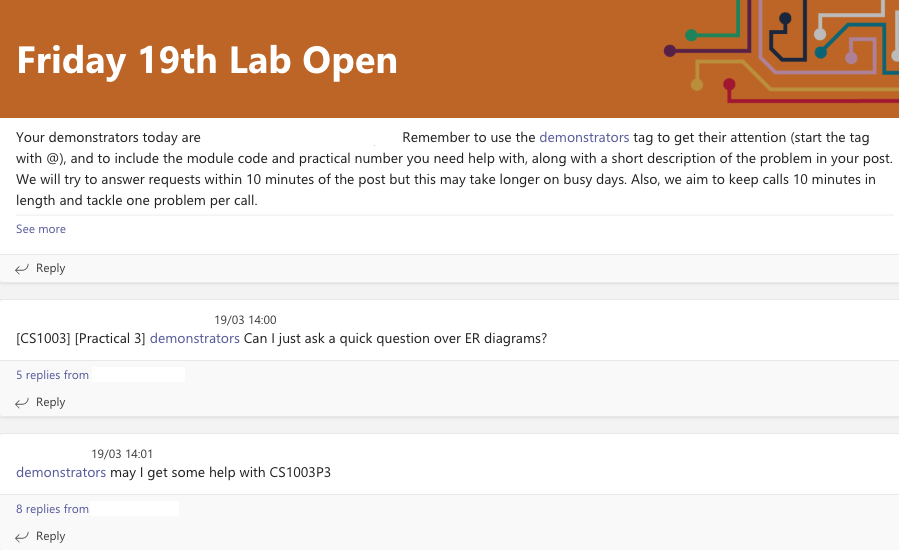
\includegraphics[width=\textwidth]{2context/images/teams1.png} 
    \caption{An example of the first iteration process of managing online labs.}
  \label{fig:teamsone}
\end{figure}

The second iteration of the system was created by using a Power Automate Flow to create an entry in a Sharepoint List when students posted an issue request to the channel. Class demonstrators used the list to show the chronological order of requests, see which demonstrator was handling each request and to mark requests as resolved. This intermediate iteration addressed most of the major issues from the first iteration, however had its own problems. There could be a delay of up to 15 minutes between the student posting in the teams channel and the request appearing on the Sharepoint List. This delay would be forgiveable in the busier labs, however is clearly unacceptable for the first 15 minutes of labs or for days on which there were fewer requests.

The third, and current, iteration of the current system uses a form input (see Figure \ref{fig:form}). This is accessed using a `Request Form' tab in the Microsoft Teams \cite{teams} CS1000 Labs team. 

\FloatBarrier
\begin{figure}[H]
  \centering
  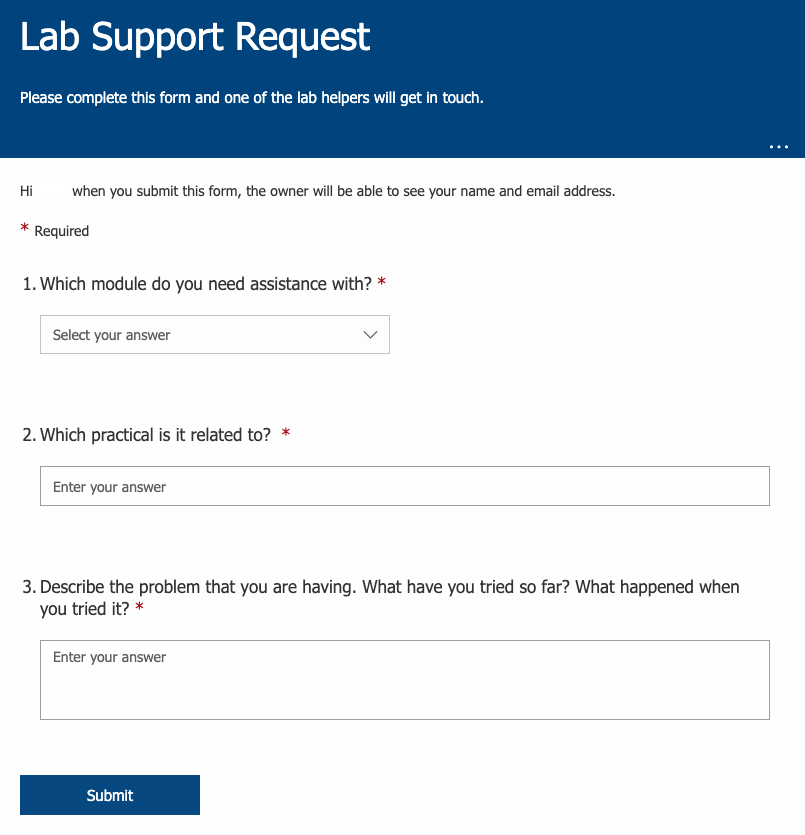
\includegraphics[width=0.85\textwidth]{2context/images/teams2a.png}
  \caption{The request form from the second iteration process of managing online labs.}
      \label{fig:form}
\end{figure}

The form uses Power Automate \cite{pauto} to post (see Figure \ref{fig:privteam}) on a private demonstrator team channel (used only to create a notification for class demonstrators) and add the form data to a Microsoft List \cite{lists}.

\FloatBarrier
\begin{figure}[H]
  \centering
  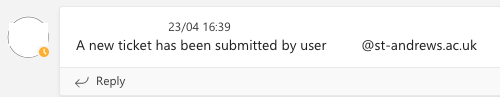
\includegraphics[width=0.6\textwidth]{2context/images/teams2b.png}
  \caption{The format of posts on the private demonstrator channel used to create notifications.}
  \label{fig:privteam}
\end{figure}

On this real-time collaborative form, class demonstrators can assign themselves to students' requests before they make contact with the student through Microsoft Teams \cite{teams}. The lab lead would also contact students by email if their request was missed, because there were too many requests to deal with during the time, or if the request was made outside of manned lab hours. The activity diagram below (see Figure \ref{fig:activdiagram}) shows the workflow for the current system during an open lab.

\FloatBarrier
\begin{figure}[H]
  \centering
  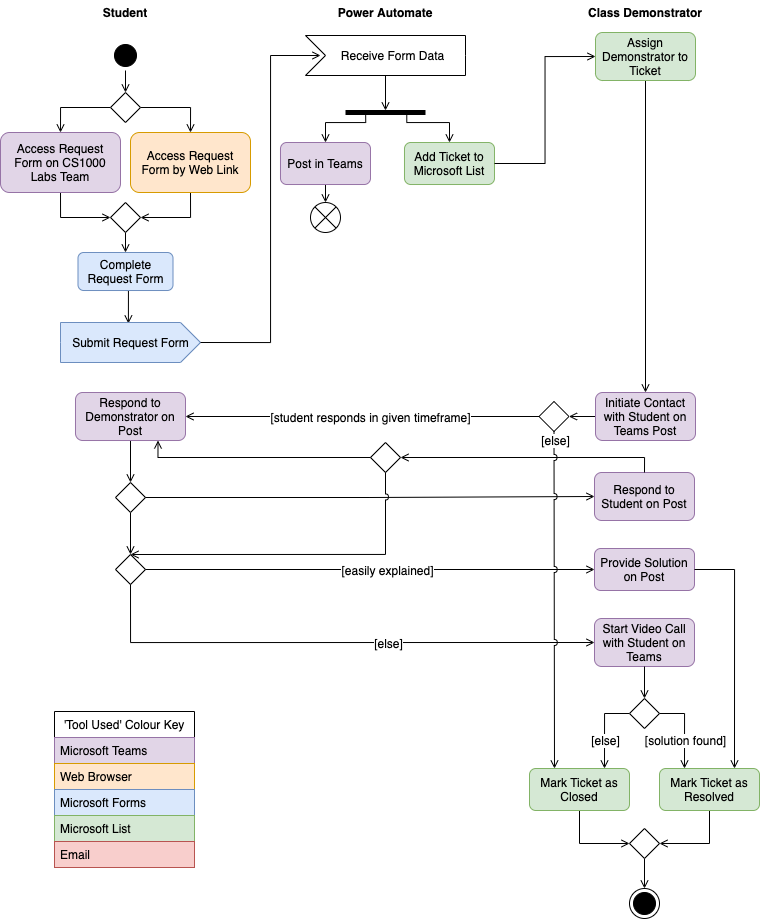
\includegraphics[width=\textwidth]{2context/images/activityRevised.png}
  \caption{\gls{uml} Activity diagram for existing method of managing student online lab request when lab is open.}
  \label{fig:activdiagram}
\end{figure}

\newpage
\section{Queue Management Tools}

Queue management tools are tools that all you to sign-in, be assigned a place in a queue and get a notification when you have reached the head of the queue. They can be be used for accessing a digital or physical resource.

ClassroomQ \cite{classroomq} is a good example of an existing queue management tool applied to an educational context. It offers a very simple system, where a teacher can create a classroom which students can join, type a message and hit an `Assistance Needed' button to join the queue of students who need help. The basic process is shown below.

Firstly, the teachers start a classroom session (see Figure \ref{fig:cqstart}).

\FloatBarrier
\begin{figure}[H]
  \centering
  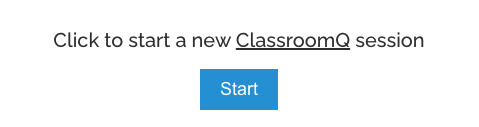
\includegraphics[width=0.5\textwidth]{2context/images/cq1.png}
  \caption{Teacher's screen when a class has not been started.}
  \label{fig:cqstart}
\end{figure}

The classroom is created, showing the class code which students can use to join (see Figure \ref{fig:cqstart}).

\FloatBarrier
\begin{figure}[H]
  \centering
  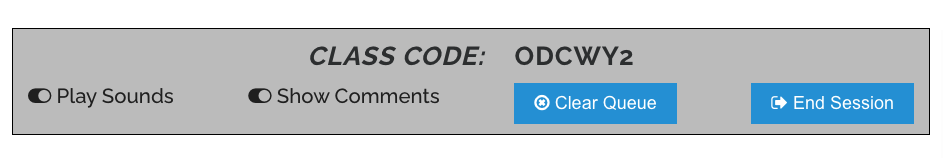
\includegraphics[width=0.75\textwidth]{2context/images/cq2.png}
  \caption{Real time classroom queue, showing class join code and current requests.}
  \label{fig:cqcode}
\end{figure}

Students join by entering their name and class code (see Figure \ref{fig:cqjoin}).

\FloatBarrier
\begin{figure}[H]
  \centering
  
\includegraphics[width=0.5\textwidth]{2context/images/cq3.png}
  \caption{Student join page, showing sample class code and name.}
  \label{fig:cqjoin}
\end{figure}

One students have joined the class, they are able to input details of their problem in the comment section and then click the `Assistance Needed' button to join the queue (see Figure \ref{fig:cqbutton}).

\FloatBarrier
\begin{figure}[H]
  \centering
  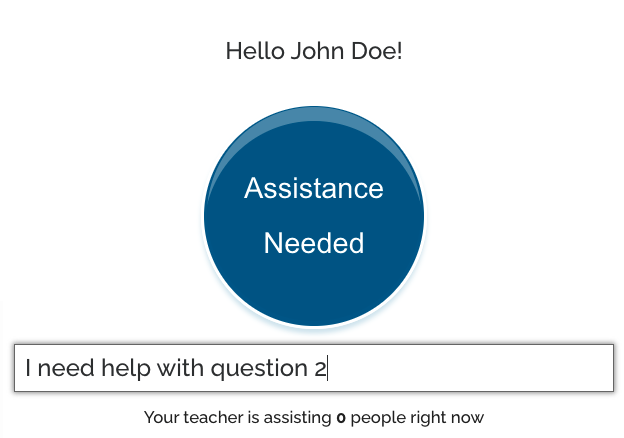
\includegraphics[width=0.5\textwidth]{2context/images/cq4.png}
  \caption{Student help request page.}
  \label{fig:cqbutton}
\end{figure}

Once the student has joined the queue, they are shown a page which allows them to cancel their request whilst showing real time information about their position in the queue (see Figure \ref{fig:cqbutton2}).

\FloatBarrier
\begin{figure}[H]
  \centering
  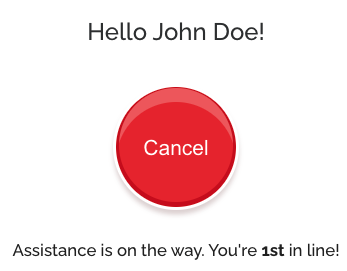
\includegraphics[width=0.5\textwidth]{2context/images/cq5.png}
  \caption{Student page after posting help request.}
  \label{fig:cqbutton2}
\end{figure}

The teacher is then able to see an ordered view of the student's requests in on the class page (see Figure \ref{fig:cqclass}).

\FloatBarrier
\begin{figure}[H]
  \centering
  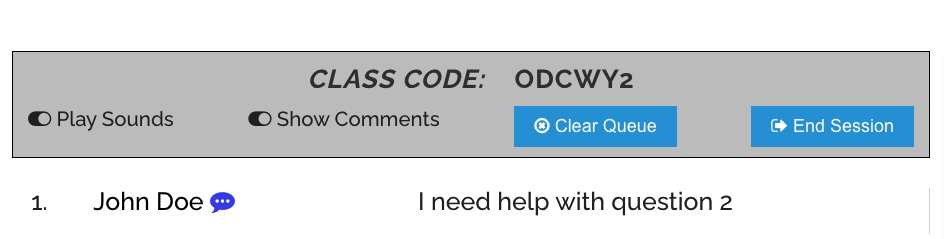
\includegraphics[width=0.75\textwidth]{2context/images/cq6.png}
  \caption{Teacher's class page view after the request has been posted.}
  \label{fig:cqclass}
\end{figure}

ClassroomQ is intended to be used with students who are physically present with the teacher in the classroom. It provides no mechanisms for online communication, assuming the communication is done in person or via some other online tool. It also assumes there is one teacher per classroom, which places an implicit limit on the number of students that can be involved in a class.

\newpage
\section{Incident Management Tools}

Incident management tools are used by IT professionals to organise, categorise and prioritise issue tickets as well as to track their resolution. These incidents can be posted by the IT professionals themselves or by other third parties who are reporting them. These tools, compared with queue management tools, offer significantly more in terms of power of automation, configurability and feature sets. However, these benefits come at the price of greater overheads in setup and maintenance. Additionally, in the context of lab management, the tool comes with an excess of complex, unnecessary and irrelevant features which result in feature fatigue \cite{ffatigue}.

Spiceworks Cloud Help Desk \cite{spiceworks} is a good example of existing incident management tools. It is a free to use, cloud-based help desk that is used by IT professionals. Traditionally, the system is used to track and manage IT issues in order to provide IT support, however the system could also be used to track and manage requests for help in our lab management domain. 

The first step in the standard Spiceworks workflow, is for the individual wishing to report an incident or issue would access a link to the help portal and enter their email address (see Figure \ref{fig:spiceemail}).

\FloatBarrier
\begin{figure}[H]
  \centering
  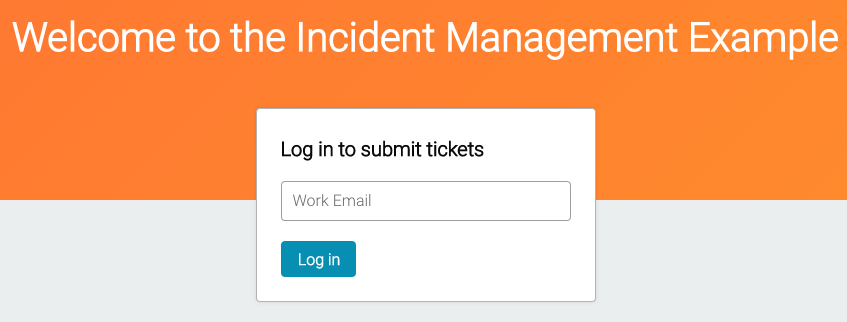
\includegraphics[width=0.7\textwidth]{2context/images/SWportalLogin.png}
  \caption{Login screen from portal link.}
  \label{fig:spiceemail}
\end{figure}

The individual would then, if authorised, receive an email link to login to the portal. This would take them to a form in which they would describe their issue (see Figure \ref{fig:spiceform}).

\FloatBarrier
\begin{figure}[H]
  \centering
  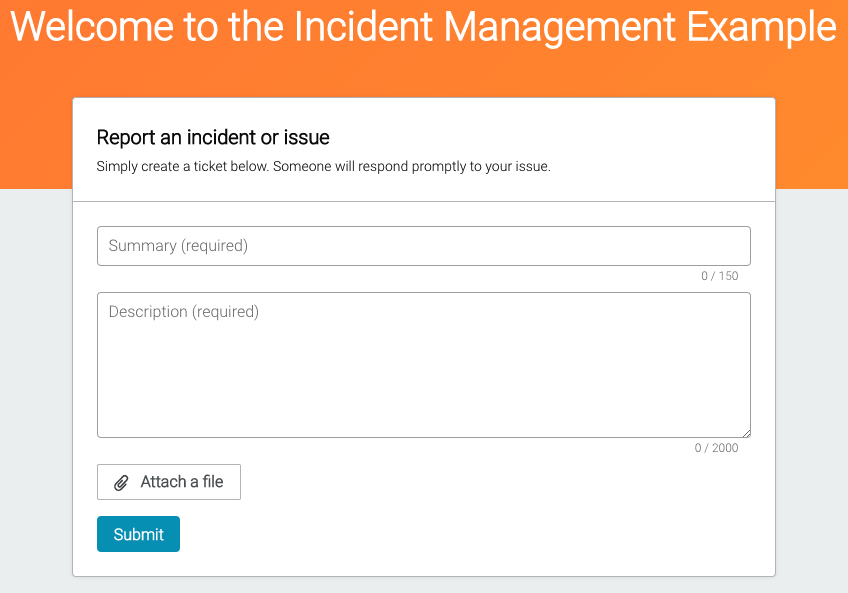
\includegraphics[width=0.75\textwidth]{2context/images/SWpostTicket.png}
  \caption{Ticket posting form, reached after login.}
  \label{fig:spiceform}
\end{figure}

The ticket would then appear on the IT help desk (see Figure \ref{fig:spicedesk}).

\FloatBarrier
\begin{figure}[H]
  \centering
  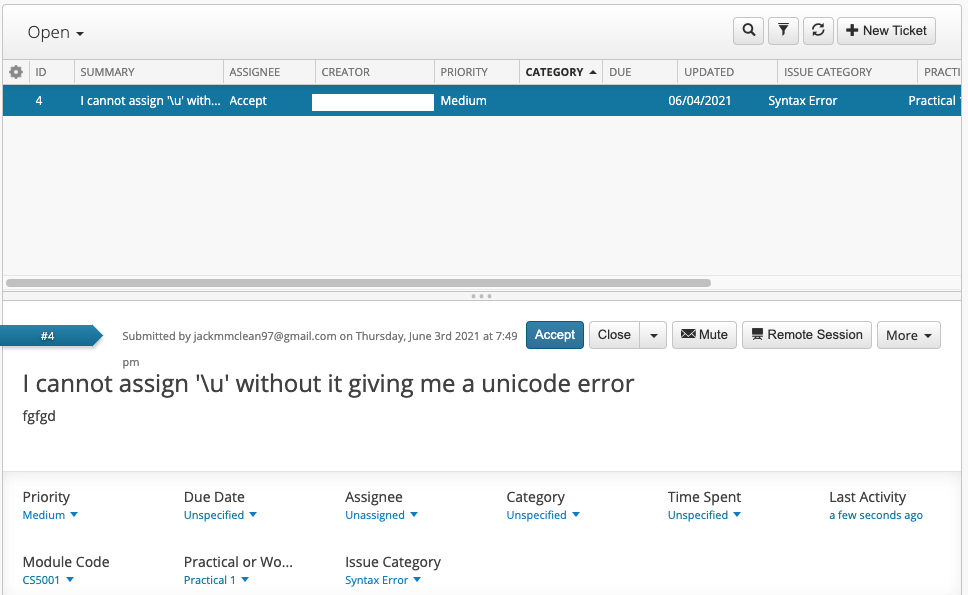
\includegraphics[width=\textwidth]{2context/images/SWticketPage.png}
  \caption{The help desk ticket page, accessible to IT Admins.}
  \label{fig:spicedesk}
\end{figure}

The IT admins are then able to respond to the ticket on Spiceworks, notifying the user by email. The IT admin can then close the ticket when the incident or issue has been resolved.

The lab management domain requires a very similar workflow, with students logging in and requesting help, and lab demonstrators responding and resolving student problems. Spiceworks also allows customisation of the incident report portal page and form categories, meaning that fields could be added for students to specify module code and practical number when posting a ticket about the issue they are facing.

